\section{Parameter optimization}

The results after the simple approach (random choice of the parameter [either usual value or complete random]) can give good result but can also give under expectation ones depending on the method used.

Thus we now try to optimize a parameter used for each methods in order to find the best value to use each time. The data used will be the training set split in two and randomised. The first new set will be the new training set and the second the validation one (for calculating the error). The following results are caluclated with the testing set.

\subsection{SVM}

On this subsection, the svms will be calculated using the function auto-train and a kfold segmentation of two (one is not accepted by the function). The dataset used is not the split one.
For the stopping point of the algorithm the max iteration and the epsilon accuracy will be used. They will vary depending on the kernel used.

\subsubsection{linear}

The first type of model used was the linear one. The stopping criteria was of either a 1000000 iterations or 0.001 for epsilon.

Results :
\begin{itemize}
  \item Correct classification : 90.65\%;
  \item Wrong classification : 9.35\%;
  \item False positive non ad : 9.07\%;
  \item False positive ad : 0.29\%.
\end{itemize}

The final selected parameter is the following : 0.5 for C. As we can see there is improvement within the results, we go from 81.87\% of correct classification to 90.65\%.

\subsubsection{Polynomial}

For this one, the number of itertion was lowered down to 100000 because the time required for the optimization was too long.

Results :
\begin{itemize}
  \item Correct classification : 94.62\%;
  \item Wrong classification : 5.38\%;
  \item False positive non ad : 4.53\%;
  \item False positive ad : 0.85\%.
\end{itemize}

The final parameters were the following ones :
\begin{itemize}
  \item degree : 343;
  \item gamma : 0.00001;
  \item coef0 : 19.6;
  \item C : 0.5.
\end{itemize}

Here we can see a great improvement within the results. we get almost no error on the false positive ads.
\subsubsection{Radial Basis Function}

We kept 100000 iterations.

Results :
\begin{itemize}
  \item Correct classification : 91.78\%;
  \item Wrong classification : 8.22\%;
  \item False positive non ad : 7.65\%;
  \item False positive ad : 0.57\%.
\end{itemize}

The final parameters were the following ones :
\begin{itemize}
  \item gamma : 0.00015;
  \item C : 312.5.
\end{itemize}


\subsubsection{Sigmoid}

Still a 100000 iterations

Results :
\begin{itemize}
  \item Correct classification : 83.85\%;
  \item Wrong classification : 16.15\%;
  \item False positive non ad : 16.15\%;
  \item False positive ad : 0\%.
\end{itemize}

The final parameters were the following ones :
\begin{itemize}
  \item gamma : 0.00015;
  \item coef0 : 0.1;
  \item C : 0.5.
\end{itemize}

Here we can see no improvement in the model, the model is still putting all the prediction in one class.

\subsection{Neural Network}

  Here we keep the same architecture for the neural network. For this model only the number of cell in the hidden layer will be optimized, not the number of hidden layer (doc here). And the data will be randomized before use. The result shown are with the best parameter each time.

  Results :
  \begin{itemize}
    \item Correct classification : 91.22\%;
    \item Wrong classification : 8.78\%;
    \item False positive non ad : 6.80\%;
    \item False positive ad : 1.983\%.
  \end{itemize}

  The best number of cells for the hidden layer was of 50 as we can see on the following figure

  \begin{figure}[h]
   \centering
   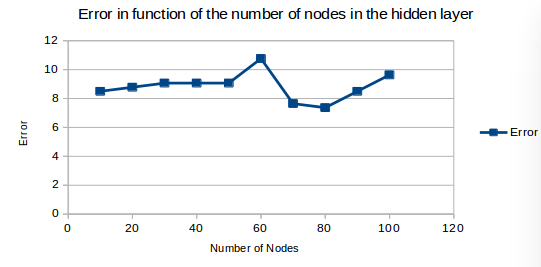
\includegraphics[scale=0.5]{../data/images/NNPO.png}
   \caption{Error depending on the number of cells in the hidden layer.}
  \end{figure}

\subsection{Random forest}

For the random forrest the only parameter optimized was the number of variable randomly selected. Here the optimization is only carried out on one of the parameter but it could be easely done on the other one. Also since it would only add calculation time this will not be done.

Results :
\begin{itemize}
  \item Correct classification : 91.22\%;
  \item Wrong classification : 8.78\%;
  \item False positive non ad : 8.22\%;
  \item False positive ad : 0.57\%.
\end{itemize}

The following figure show the error against the selected parameter to optimize.

\begin{figure}[h]
 \centering
 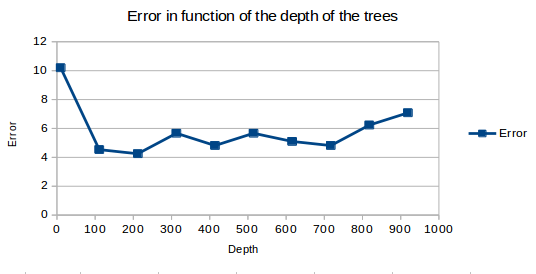
\includegraphics[scale=0.5]{../data/images/RFPO.png}
 \caption{Error depending on the number of variable randomly selected.}
\end{figure}
